\documentclass[a4paper]{scrartcl}

\usepackage[utf8]{inputenc}
\usepackage[ngerman]{babel}

\usepackage{url,amssymb,mathrsfs,enumerate,dsfont}
\usepackage[space,extendedchars]{grffile}
\usepackage{verbatim}
\usepackage{listings}
\usepackage{geometry}
\usepackage{tikz}
\usepackage{etoolbox}
\usetikzlibrary{automata,arrows}
\usepackage{subfigure}
\usepackage[ngerman]{babel}
\usepackage{hyperref}
\usepackage{blindtext}
\usepackage{framed}
\usepackage{paralist}
\usepackage{multirow} 
\usepackage{amsmath}
\usepackage{algorithm}
\usepackage[noend]{algpseudocode}

\def\ojoin{\setbox0=\hbox{$\bowtie$}%
  \rule[-.02ex]{.25em}{.4pt}\llap{\rule[\ht0]{.25em}{.4pt}}}
\def\leftouterjoin{\mathbin{\ojoin\mkern-5.8mu\bowtie}}
\def\rightouterjoin{\mathbin{\bowtie\mkern-5.8mu\ojoin}}
\def\fullouterjoin{\mathbin{\ojoin\mkern-5.8mu\bowtie\mkern-5.8mu\ojoin}}

\usetikzlibrary{arrows,shapes, automata}
\setkomafont{disposition}{\normalfont\bfseries}
\setlength\parindent{0pt}

\lstset
{ %Formatting for code in appendix
    language=c,
    basicstyle=\footnotesize,
    numbers=left,
    stepnumber=1,
    showstringspaces=false,
    tabsize=4,
    breaklines=true,
    breakatwhitespace=false,
}

\title{Mathematik für Informatiker \\ Kombinatorik, Stochastik und Statistik}
\subtitle{Übungsblatt 7}
\author{Tom Paßberg , Iain Dorsch}
\date{}
\begin{document}

\maketitle

\newpage

\section*{Aufgabe 1}
\subsection*{a)}
Wir erreichen $\binom{n}{2}$ Vergleiche wenn wir als Pivot Element immer das Kleinste Element der Eingabe Wählen. \\
Wir Testen diese Ausage mit einem Rust Programm, die Vergleiche, die zur Ermittlung des Minimums benötigt werden, werden nicht mitgezählt.
Die gemessene Laufzeit k<ann in einem Randomisierten Quicksort mit sehr ungünstiger Pivot-Wahl auftreten. 

\textbf{Algorithmus in Rust:}
\begin{lstlisting}
fn main() {
	let input = vec![56,64,58,61,75,86,17,62,8,50,87,99,67,10,74];

	let (_, num_comparisons) = bad_quicksort(input);

	println!("Number of comparisons: {}", num_comparisons);
}

fn bad_quicksort(mut vec: Vec<i32>) -> (Vec<i32>, u64) {
	if vec.len() <= 1 {
		return (vec, 0);
	}
	let num_comparisons = vec.len() as u64 - 1;
	let pivot = *vec.iter().min().unwrap();
	vec.retain(|&x| x != pivot);
	let (left, right) = vec.into_iter().partition(|&x| x < pivot);

	let (mut result, count) = bad_quicksort(left);
	let (right_result, right_count) = bad_quicksort(right);
	result.push(pivot);
	result.extend(right_result);
	(result, count + right_count + num_comparisons)
}
\end{lstlisting}

\textbf{Ausgabe:}
\begin{lstlisting}
Number of comparisons: 105
\end{lstlisting}
Die Wahl der Pivotelemnte erfüllt die Anforderung $105 = \binom{15}{2}$

\subsection*{b)}
Wenn wir als Pivot Element immer das Median der Eingabe Wählen erhalten wir die best case Laufzeit.
Wir zählen die Vergleiche zur Ermittlung des Medians nicht mit, die Laufzeit ist also die best case Laufzeit eines Randomisierten Quicksort Algorithmus.

Wir testen die Aussage mit einem Rust Programm.
\begin{lstlisting}
fn good_quicksort(mut vec: Vec<i32>) -> (Vec<i32>, u64) {
	if vec.len() <= 1 {
		return (vec, 0);
	}
	let num_comparisons = vec.len() as u64 - 1;
	let pivot = median(&vec);
	vec.retain(|&x| x != pivot);
	let (left, right) = vec.into_iter().partition(|&x| x < pivot);

	let (mut result, count) = good_quicksort(left);
	let (right_result, right_count) = good_quicksort(right);
	result.push(pivot);
	result.extend(right_result);
	(result, count + right_count + num_comparisons)
}
\end{lstlisting}
Ausgabe:
\begin{lstlisting}
Number of comparisons: 34
\end{lstlisting}
Die Wahl des Medians als Pivot Element erfüllt die Anforderung $34 < 15 \cdot \ln(15)$

\section*{Aufgabe 2}
Als Laufzeit betrachten wir die Anzahl der Multiplikationen.\\
\begin{enumerate}
\item [a)] 
\begin{align}
&A \cdot x\\
= &\left(\sum_{j=1}^{n} a_{ij}x_j\right)_{i=1..n}
\end{align}
Die Summenformel wird $ n $ mal berechnet. 
Wir substituieren $a_{ij}x_j$ durch $1$, damit zählen wir die Anzahl der multiplikations Operationen
\begin{align}
&n\cdot\left(\sum_{j=1}^{n} 1\right)\\
= &n\cdot n\\
= &n^2
\end{align}

\item [b)]
\begin{align}
&A \cdot B\\
= &\left(\sum_{j=1}^{n} a_{ij}x_{jk}\right)_{i,k=1..n}
\end{align}
Die Summenformel wird $ n \cdot n $ mal berechnet (für $i,k \in 1..n$).
Wir substituieren $a_{ij}x_{jk}$ durch 1 (zähle die Anzahl der multiplikations Operationen):
\begin{align}
&n\cdot\left(n\cdot\left(\sum_{j=1}^{n} 1\right)\right)\\
= &n\cdot n\cdot n\\
= &n^3\\
\end{align}
\item [c)]
Sei $ C = A \cdot B $, dann gilt 
\begin{align*}
	C \cdot x &= A \cdot (B \cdot x)\\
\end{align*}
Wir testen für zufällige $x$ ob die Gleichung gilt. Einen vektor mit einer Matirx zu multiplizieren ist eine Operation der Laufzeit $\mathcal{O}(n^2)$.
Der nachfolgende Rust Code testet die Gleichung für zufällige $x$ in $O(n^2)$:
\begin{lstlisting}
fn monte_carlo_test(A: &Matrix, B: &Matrix, C: &Matrix) -> bool {
	for i in 0..10 {
		let x = (0..C.cols).map(|_| random::<f32>() as f64).collect::<Vec<f64>>();
		let P = C.vec_multiply(&x);
		let Q = A.vec_multiply(&B.vec_multiply(&x));
		if P != Q {
			return false;
		}
	}
	true
}
\end{lstlisting}

\end{enumerate}

\newpage
\section*{Aufgabe 3}
\subsection*{a)}

\textbf{Algorithmus in Rust:} 
\begin{lstlisting}
fn quicksort(vec: Vec<i32>) -> (Vec<i32>, u64) {
	if vec.len() <= 1 {
		return (vec, 0);
	}
	let num_comparisons = vec.len() as u64 - 1;
	let mut iter = vec.into_iter();
	let pivot = iter.next().unwrap();
	let (left, right) = iter.partition(|&x| x < pivot);

	let (mut result, count) = quicksort(left);
	let (right_result, right_count) = quicksort(right);
	result.push(pivot);
	result.extend(right_result);
	(result, count + right_count + num_comparisons)
}
\end{lstlisting}
Als pivot-Element wird immer das erste Element der Eingabe gewählt. Die Funktion gibt ein Tupel zurück, bestehend aus dem sortierten Vektor und der Anzahl der Vergleiche. 
Wir zählen nur die Vergleiche zwischen Listenelementen, nicht den Vergleich der Länge der Liste mit der Zahl 1 (Für die assymptitische Laufzeit macht das keinen Unterschied).

\textbf{Funktionsaufruf:}
\begin{lstlisting}
fn main() {
	let input = vec![3, 2, 1, 7, 6, 4, 5, 8, 10, 9];
	let (sorted, count) = quicksort(input);
	println!("Sorted: {:?}\nComparisions: {}", sorted, count);
}
\end{lstlisting}

\textbf{Ausgabe:}
\begin{lstlisting}
Sorted: [1, 2, 3, 4, 5, 6, 7, 8, 9, 10]
Comparisions: 20
\end{lstlisting}

\subsection*{b)}
\textbf{Daten erzeugen:}
\begin{lstlisting}
fn main() {
	let mut workbook = Workbook::new();
	let worksheet = workbook.add_worksheet();

	worksheet.write(0, 0, "#Elements").unwrap();
	worksheet.write(1, 0, "#Comparisions").unwrap();

	let sample_size = 20;
	for i in 1..=25 {
		let count_sum = (0..sample_size).into_par_iter().map(|_| {
			let mut vec = Vec::with_capacity(2usize.pow(i));
			for _ in 0..2usize.pow(i) {
				vec.push(rand::random::<i32>());
			}
			let mut truth = vec.clone();
			truth.sort_unstable();
			
			let (sorted, count) = quicksort(vec);
			// teste ob das Ergebnis korrekt ist
			assert_eq!(sorted, truth);
			count
		}).sum::<u64>();

		// berechne den Durchschnitt der Vergleiche
		let count = (count_sum as f32 / sample_size as f32) as i32;
		
		println!("Elements: {:10}, Comparisions: {:13}", 2usize.pow(i), count);
		
		// Schreibe Ergebiss in Excel Datei
		worksheet.write(0, i as u16, 2usize.pow(i) as i32).unwrap();
		worksheet.write(1, i as u16, count).unwrap();
	}
	workbook.save("quicksort.xlsx").unwrap();
}
\end{lstlisting}

\textbf{Grafische Darstellung der Ausgabe:}
\begin{figure}[H]
	\centering
	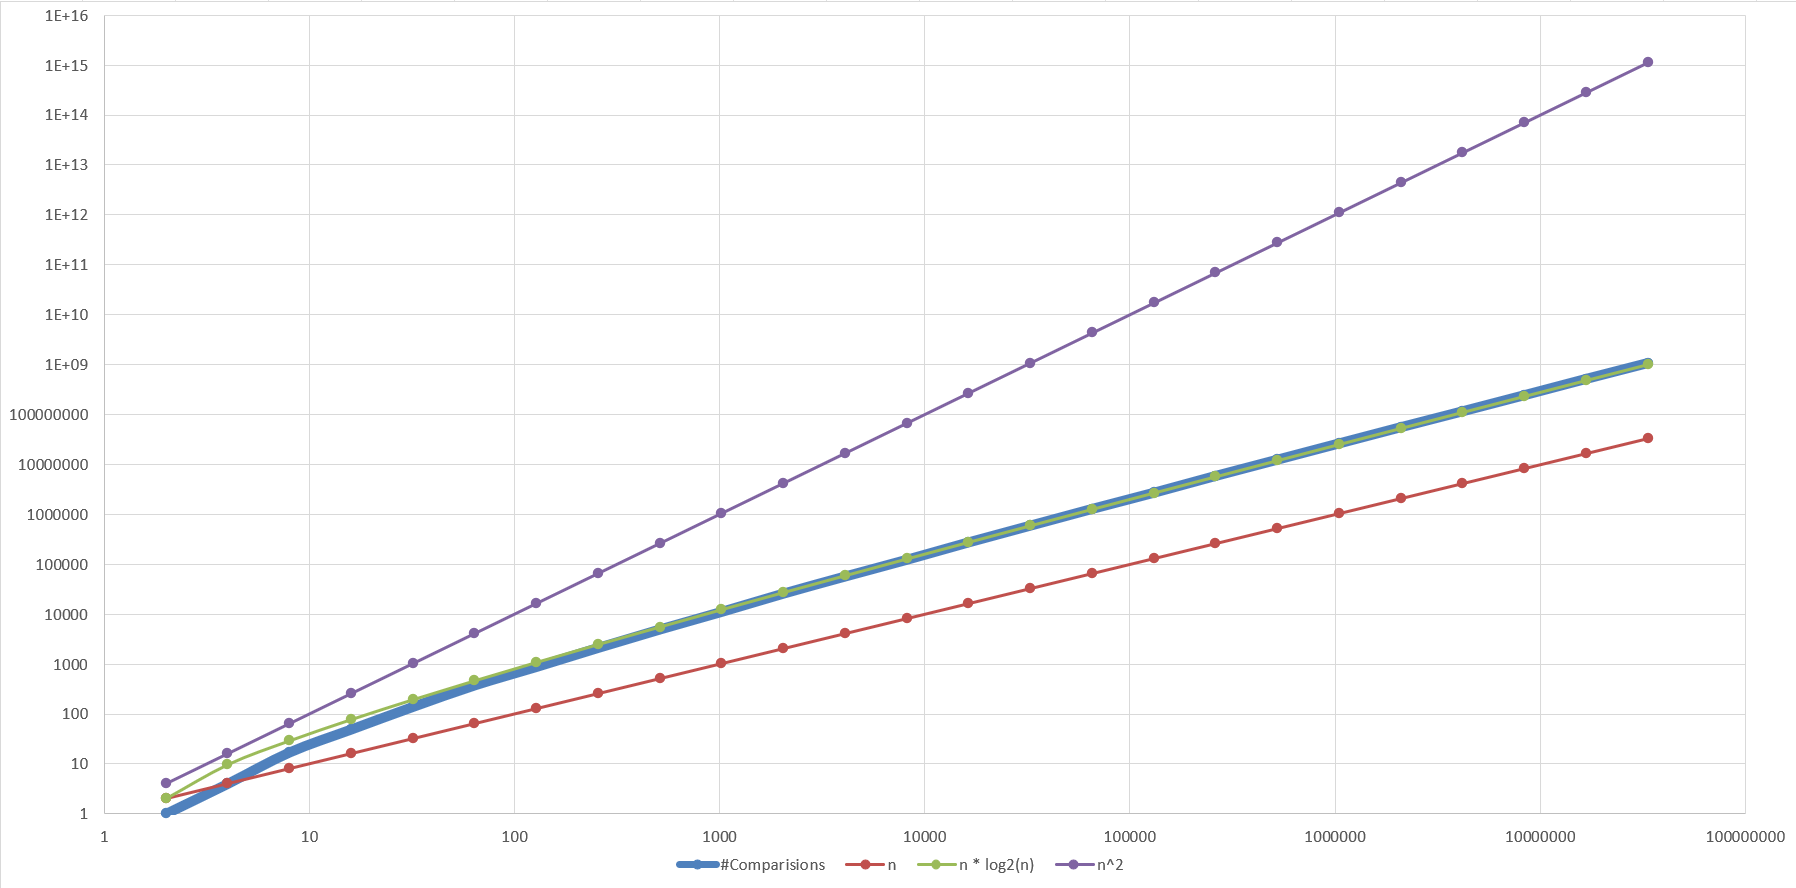
\includegraphics[width=1.0\textwidth]{graph.png}
\end{figure}
Die Laufzeit verhält sich wie erwartet mit $\mathcal{O}(n \log n)$.

\end{document}